\documentclass[10pt]{beamer}

%% Based on the original theme by Matthias Vogelgesang
%% Merged template: ie.tex color palette + IAAE.tex presentation roadmap

\usetheme[progressbar=frametitle]{metropolis}
\usepackage{appendixnumberbeamer}

\usepackage{booktabs}
%\usepackage[scale=2]{ccicons} % removed: unused; not installed in all TeX distros

\usepackage{pgfplots}
\usepgfplotslibrary{dateplot}

\usepackage{xspace}
\usepackage{xcolor}
\usepackage{lmodern}
\usepackage{amsmath}
\usepackage{amssymb}
\usepackage{bm}
\newcommand{\themename}{\textbf{\textsc{metropolis}}\xspace}

%%%%%%%%%%%%%%%%%%%%%%%%%%%%
%%  Theme Adjustments     %%
%%%%%%%%%%%%%%%%%%%%%%%%%%%%
\definecolor{CanvasBG}{HTML}{FAFAFA}

% Color palette (from ie.tex)
\definecolor{UnccGreen}{HTML}{005035}
\definecolor{UnccLightGreen}{HTML}{C3D7A4}
\definecolor{UnccGold}{HTML}{A49665}
\definecolor{UnccOrange}{HTML}{F3901D}
\definecolor{UnccLightYellow}{HTML}{899064}
\definecolor{UnccBlue}{HTML}{007377}
\definecolor{UnccPink}{HTML}{DE3A6E}
\definecolor{White}{HTML}{FFFFFF}
\definecolor{LightGray}{HTML}{F1E6B2}

\setbeamercolor{frametitle}{bg=white, fg=UnccGreen}
\setbeamercolor{progress bar}{bg=UnccGold, fg=UnccGreen}
\setbeamercolor{alerted text}{fg=UnccOrange}

\setbeamercolor{block title}{bg=UnccGreen, fg=White}
\setbeamercolor{block title example}{bg=UnccBlue, fg=White}
\setbeamercolor{block title alerted}{bg=UnccPink, fg=White}
\setbeamercolor{block body}{bg=LightGray}

\metroset{titleformat=smallcaps, progressbar=foot}

\makeatletter
\setlength{\metropolis@progressinheadfoot@linewidth}{2pt}
\setlength{\metropolis@titleseparator@linewidth}{2pt}
\setlength{\metropolis@progressonsectionpage@linewidth}{2pt}
\makeatother
%%%%%%%%%%%%%%%%%%%%%%%%%%%%


\title{The International Credit Channel of U.S. Financial Shocks}
\subtitle{Discussion of Cesa-Bianchi \& Sokol (2022)}
\date{\today}
\author{Mansi Mate}
\institute{Advanced Macro \\ Graduate Institute}

\begin{document}

\maketitle

%===============================================
\section{Introduction}
%===============================================

%-----------------------------------------------
% SLIDE 1 -- Motivation / Research question
%-----------------------------------------------
\begin{frame}{Is there an international credit channel beyond monetary policy?}
\begin{itemize}
    \item U.S. monetary policy transmits across borders: synchronised movements in credit spreads, capital flows, and asset prices -- the \textbf{International Credit Channel} \textcolor{gray}{\scriptsize(Rey, 2016)}.
    \vspace{0.3em}
    \item U.S. shocks affect net worth of agents worldwide $\Rightarrow$ co-movement of financial conditions.
    \vspace{0.3em}
    \item \textbf{This paper:} does the same credit channel transmit \emph{financial} shocks internationally -- and how does it compare to monetary policy (MP) and central-bank information (CBI) shocks?
\end{itemize}
\end{frame}


%-----------------------------------------------
% SLIDE 2 -- Financial shocks and business cycles
%-----------------------------------------------
\begin{frame}{Financial shocks explain business cycles}
\begin{itemize}
    \item \textbf{Financial shocks}, broadly defined: exogenous changes to the net worth of financially constrained agents, or to their degree of risk aversion.
    \vspace{0.4em}
    \item \textbf{Identification is hard} -- they mimic
    \begin{itemize}
        \item central-bank information shocks, and
        \item aggregate-demand shocks.
    \end{itemize}
    \vspace{0.4em}
    \item Need an approach that \textbf{separately identifies} financial shocks to assess their domestic and international effects.
\end{itemize}
\end{frame}


%-----------------------------------------------
% SLIDE 3 -- Novel Identification
%-----------------------------------------------
\begin{frame}{Novel identification: combining IVs and sign restrictions}
\begin{enumerate}
    \item \textbf{Step 1.} Jointly identify MP and CBI shocks via high-frequency FOMC surprises \textcolor{gray}{\scriptsize(Jarocinski \& Karadi, 2020)} and use them as \textbf{external instruments}.
    \vspace{0.4em}
    \item \textbf{Step 2.} Conditional on Step 1, derive a \textbf{minimum set of sign restrictions} from theory that uniquely identify a broad class of financial shocks.
\end{enumerate}
\vspace{0.6em}
\pause
\textcolor{blue}{$\boldsymbol{\Rightarrow}$} Embedded in a \textbf{two-country SVAR} for the U.S. and U.K.\\
\textit{(large small-open economy, floating ER, inflation targeting, well-developed financial sector).}
\end{frame}


%-----------------------------------------------
% SLIDE 4 -- Main Results
%-----------------------------------------------
\begin{frame}{Main results}
\begin{enumerate}
    \item \textbf{Existence of an ICC in U.S.\ financial-shock transmission} -- U.S.\ shocks tighten domestic credit, transmit to U.K.\ spreads, and lower U.K.\ real activity.\\
    {\scriptsize\textcolor{gray}{Extends Helbling et al.\ (2011), Eickmeier \& Ng (2015) -- we pin down the credit-channel mechanism.}}
    \vspace{0.3em}
    \item \textbf{U.S.\ MP also transmits internationally via credit spreads} -- narrowing the U.S.--U.K.\ spread differential.\\
    {\scriptsize\textcolor{gray}{Complements Rey (2016), Passari \& Rey, Gerko \& Rey (2017), Kalemli-\"Ozcan (2019) -- we control for CBI.}}
    \vspace{0.3em}
    \item \textbf{CBI shocks generate cross-country spillovers via the ICC} -- a positive U.S. outlook compresses U.S.\ spreads and transmits quickly to the U.K.\\
    {\scriptsize\textcolor{gray}{Complements Stavrakeva \& Tang (2019), Miranda-Agrippino \& Rey (2020), Jarocinski (2020).}}
\end{enumerate}
\end{frame}


%-----------------------------------------------
% ROADMAP
%-----------------------------------------------
\begin{frame}{Presentation Roadmap}
\begin{enumerate}
    \item \textbf{Introduction}
    \vspace{0.4em}
    \item \textbf{Econometric Approach}
    \begin{itemize}
        \item Identification strategy: IVs + sign restrictions
        \item Two-country SVAR
        \item Identifying financial shocks
    \end{itemize}
    \vspace{0.4em}
    \item \textbf{Data \& Results}
    \begin{itemize}
        \item Domestic and international transmission
    \end{itemize}
    \vspace{0.4em}
    \item \textbf{Mechanism}
    \vspace{0.4em}
    \item \textbf{Conclusion}
\end{enumerate}
\end{frame}


%===============================================
\section{Econometric Approach}
%===============================================

%-----------------------------------------------
% SLIDE 5 -- Identification strategy (SVAR + IV)
%-----------------------------------------------
\begin{frame}{Identification strategy}
\textbf{Standard SVAR:}
\begin{equation*}
y_t = \Phi(L)\, y_{t-1} + B\, e_t, \qquad \mathbb{E}[e_t e_t'] = I_n
\end{equation*}
\vspace{-0.6em}
\begin{itemize}\scriptsize
    \item $y_t$: $n\times 1$ vector of observables; $e_t$: unobserved structural shocks; $B$: impact matrix; $u_t = B e_t$.
    \item Identification problem: $\Sigma_u = BB'$ gives $n(n+1)/2$ equations but $n^2$ unknowns in $B$.
\end{itemize}
\pause
\vspace{0.3em}
\textbf{Partition into two types of shocks:}
\begin{equation*}
B = \begin{bmatrix} B^{IV} & B^{SR} \end{bmatrix}, \qquad
e_t^{IV} = (e_{1,t}',\dots,e_{k,t}')', \quad
e_t^{SR} = (e_{k+1,t}',\dots,e_{n,t}')'
\end{equation*}
\vspace{-0.4em}
\begin{itemize}\scriptsize
    \item $k<n$ shocks identified by \textbf{external instruments} -- $B^{IV}$ is $n\times k$.
    \item Remaining $n-k$ shocks identified by \textbf{sign restrictions} -- $B^{SR}$ is $n\times(n-k)$.
    \item Here $k=2$: one monetary-policy shock and one CB-information shock.
\end{itemize}
\pause
\vspace{0.3em}
\textbf{External instruments:} $z_t = (z_{1,t}',\dots,z_{k,t}')'$
\begin{equation*}
\mathbb{E}[z_t e_t^{IV\prime}] \neq 0, \qquad \mathbb{E}[z_t e_t^{SR\prime}] = 0
\end{equation*}
{\scriptsize MP surprise + CBI surprise from high-frequency Fed-Funds futures around FOMC announcements \textcolor{gray}{(Jarocinski \& Karadi, 2020)}.}
\end{frame}


%-----------------------------------------------
% SLIDE 6 -- Combining sign + IV
%-----------------------------------------------
\begin{frame}{Combining sign restrictions and external instruments}
Rely on economic theory to pin down a \textbf{unique} set of sign restrictions consistent with $e_t^{SR}$.
\vspace{0.5em}
\begin{align*}
\Sigma_u &= BB' = \begin{bmatrix} B^{IV} & B^{SR} \end{bmatrix}\begin{bmatrix} B^{IV} & B^{SR} \end{bmatrix}' \\[0.3em]
\Sigma_u &= CC' = CQQ'C' = (CQ)(CQ)', \quad \text{where $QQ' = I$, $C$ is Cholesky of $\Sigma_u$} \\[0.3em]
CQ &= \begin{bmatrix} B^{IV} & B^{SR} \end{bmatrix} = B
\end{align*}
\pause
\textbf{Algorithm} \textcolor{gray}{\scriptsize(Rubio-Ramirez et al., 2010)}:
\begin{enumerate}\scriptsize
    \item Find $q$ such that $Cq = B^{IV}$ -- IV pins down the first $k$ columns exactly.
    \item Complete $Q$ via Gram-Schmidt over the remaining $n-k$ columns.
    \item Retain the draw if $B^{SR}$ satisfies sign restrictions; discard otherwise.
\end{enumerate}
\vspace{0.3em}
Repeat over bootstrap draws -- report 90\% credible intervals over all retained $Q$.
\end{frame}


%-----------------------------------------------
% SLIDE 7 -- Two-country SVAR
%-----------------------------------------------
\begin{frame}{A two-country SVAR}
\textbf{Setup:} U.S.\ = Foreign ($F$), U.K.\ = Home ($H$):
\begin{equation*}
\begin{bmatrix} y_t^F \\ y_t^H \end{bmatrix}
=
\begin{bmatrix} \Phi_{FF}(L) & \Phi_{FH}(L) \\ \Phi_{HF}(L) & \Phi_{HH}(L) \end{bmatrix}
\begin{bmatrix} y_{t-1}^F \\ y_{t-1}^H \end{bmatrix}
+
\begin{bmatrix} B_{FF} & B_{FH} \\ B_{HF} & B_{HH} \end{bmatrix}
\begin{bmatrix} e_t^F \\ e_t^H \end{bmatrix}
\end{equation*}
\scriptsize where $y_t = (y_t^{F\prime}, y_t^{H\prime})'$ collects $n = n_F + n_H$ endogenous variables, $e_t = (e_t^{F\prime}, e_t^{H\prime})'$ are structural shocks with $\mathbb{E}[e_t e_t']=I$, and $\Phi(L)$ is a matrix polynomial in the lag operator.
\normalsize
\vspace{0.4em}
\pause
\textbf{Block exogeneity} -- U.K. treated as a small open economy; no feedback from Home to Foreign:
\begin{equation*}
\Phi_{FH}(L) = 0 \qquad\qquad B_{FH} = 0
\end{equation*}
\vspace{-0.3em}
\begin{itemize}\scriptsize
    \item Estimate reduced form for U.S., identify $e_t^F$.
    \item Then estimate for U.K.
    \item Impact of foreign structural shocks on Home variables ($B_{HF}$): regress $u_t^H = \lambda\, e_t^F$. \\ OLS coefficients $\lambda$ capture the response of $H$ to $F$ structural shocks \textcolor{gray}{\scriptsize(Canova, 2005)}.
\end{itemize}
\end{frame}


%-----------------------------------------------
% SLIDE 8 -- Challenge
%-----------------------------------------------
\begin{frame}{Challenge: identifying financial shocks}
\begin{enumerate}
    \item \textbf{Fast-moving financial variables} $\Rightarrow$ contemporaneous zero restrictions (Cholesky) implausible; literature moved to sign restrictions.
    \vspace{0.4em}
    \item Even with sign restrictions, \textbf{financial shocks look like aggregate-demand shocks}: both lead to falling output, prices, and policy rates.
    \vspace{0.4em}
    \item \textbf{Different financial shocks look identical} to each other, with similar qualitative effects on aggregates. Separating them requires higher VAR dimensionality $\Rightarrow$ \emph{curse of dimensionality}.
\end{enumerate}
\pause
\vspace{0.6em}
\textcolor{blue}{$\boldsymbol{\Rightarrow}$} The paper shows it is possible to use a \textbf{minimum set of restrictions} to distinguish a broad class of financial shocks from a classical aggregate-demand shock.
\end{frame}


%-----------------------------------------------
% SLIDE 9 -- Solution: borrowing rate
%-----------------------------------------------
\begin{frame}{Solution: response of the borrowing rate}
Based on theoretical models with sticky prices and a financial-accelerator mechanism \textcolor{gray}{\scriptsize(Bernanke et al., 1999; Christiano et al., 2014)}:
\begin{equation*}
i_B^m = i^m + x^m
\end{equation*}
\vspace{-0.3em}
\begin{itemize}\scriptsize
    \item $i_B^m$: borrowing rate, $i^m$: government bond rate, $x^m$: credit spread.
\end{itemize}
\vspace{0.3em}
\pause
After an adverse shock, monetary policy eases ($i^m \downarrow$) but the credit spread rises ($x^m \uparrow$), so the response of $i_B^m$ is \textbf{theoretically ambiguous}. We exploit this ambiguity:
\vspace{0.5em}

\textbf{Negative financial shock:} \quad spread dominates $\Rightarrow\ x^m\!\uparrow\, >\, i^m\!\downarrow \Rightarrow \boldsymbol{i_B^m \uparrow}$

\textbf{Negative demand shock:} \quad policy rate dominates $\Rightarrow\ i^m\!\downarrow\, >\, x^m\!\uparrow \Rightarrow \boldsymbol{i_B^m \downarrow}$
\vspace{0.5em}
\pause
\textcolor{blue}{$\boldsymbol{\Rightarrow}$} The \textbf{sign of $i_B^m$} is the minimum restriction that uniquely identifies a broad class of financial shocks from aggregate-demand shocks.
\end{frame}


%-----------------------------------------------
% SLIDE 10 -- Empirical Evidence (Lehman)
%-----------------------------------------------
\begin{frame}{Empirical evidence: the Lehman moment}
\begin{center}
    {\small \textbf{Figure 1} --- Fed Funds, BAA Interest Rate, and BAA Spread}\\[0.3em]
    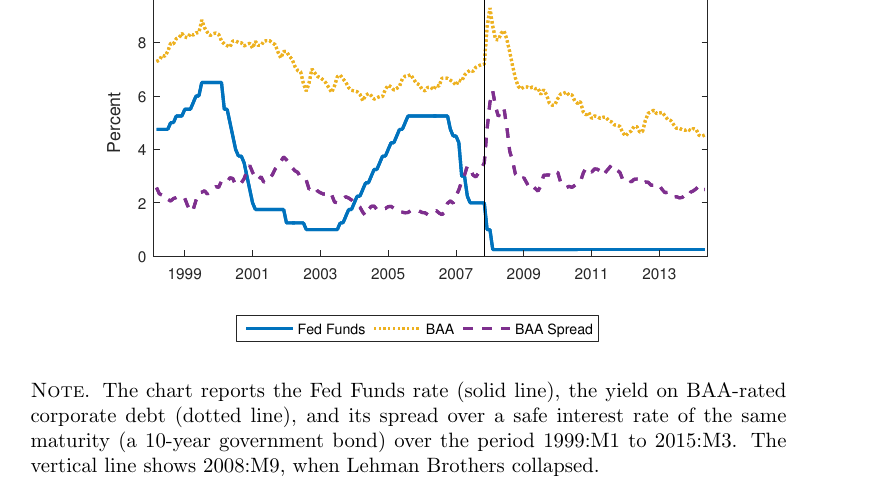
\includegraphics[width=0.8\linewidth]{images/fig1_lehman.png}
\end{center}
\vspace{-0.3em}
\begin{itemize}\small
    \item At the Lehman Brothers collapse (2008:M9): Fed cuts sharply ($i^m\!\downarrow$) -- yet the BAA spread spikes ($x^m\!\uparrow$).
    \item \textbf{Spread dominates} $\Rightarrow$ the borrowing rate \emph{rises} despite monetary easing.
\end{itemize}
\end{frame}


%===============================================
\section{Data \& Results}
%===============================================

%-----------------------------------------------
% SLIDE 11 -- Data & Estimation
%-----------------------------------------------
\begin{frame}{Data and estimation}
\begin{itemize}\small
    \item \textbf{U.S.\ VAR (Foreign):} real GDP, CPI, 1-yr government bond rate, Excess Bond Premium \textcolor{gray}{\scriptsize(Gilchrist \& Zakraj\v{s}ek, 2012)}, borrowing rate (10-yr gov bond + GZ corporate spread).
    \vspace{0.3em}
    \item \textbf{Identification of MP and CBI shocks:} following Jarocinski \& Karadi (2020), decompose high-frequency surprises in Fed-Funds futures (FF4) around FOMC announcements into a monetary-policy and an information component; use as external instruments $z_t$ in the U.S.\ VAR.
    \vspace{0.3em}
    \item \textbf{U.K.\ VAR (Home):} real GDP, CPI, 1-yr gilt rate, nominal ER (vs.\ USD), corporate bond spread; 3 lags of U.S.\ variables included as exogenous regressors (block exogeneity).
    \vspace{0.3em}
    \item \textbf{Inference:} credible intervals via wild bootstrap \textcolor{gray}{\scriptsize(Mertens \& Ravn, 2013)}.
\end{itemize}
\end{frame}


%-----------------------------------------------
% SLIDE 11b -- US Financial Shock: Domestic
%-----------------------------------------------
\begin{frame}{U.S.\ financial shock: domestic transmission}
\begin{center}
    {\small \textbf{Figure 4} --- US Financial Shock: Transmission Within the US}\\[0.3em]
    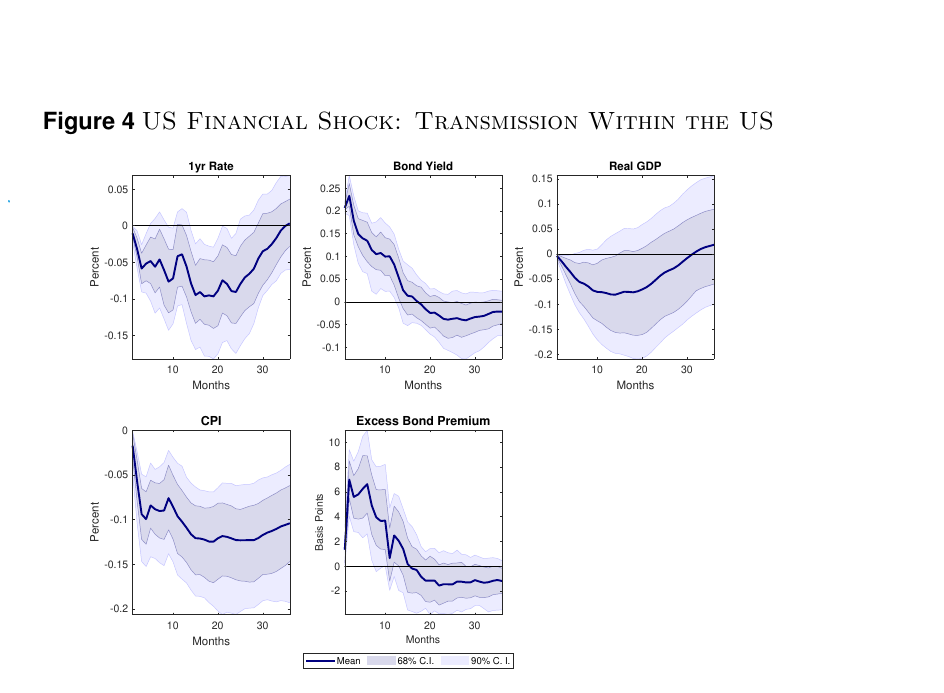
\includegraphics[width=0.85\linewidth]{images/fig4_usfin_us.png}
\end{center}
\vspace{-0.4em}
\begin{itemize}\scriptsize
    \item \textbf{1 SD} adverse financial shock: Excess Bond Premium rises ($\sim$7\,bp), real GDP contracts ($\sim$0.1\%), prices fall ($\sim$0.15\%) -- consistent with the sign restrictions.
    \item Despite \textbf{loosening} monetary policy (1-yr rate $\downarrow$ $\sim$0.1\%), credit conditions \textbf{tighten} -- the spread dominates, as the identification predicts.
\end{itemize}
\end{frame}


%-----------------------------------------------
% SLIDE 12 -- US Financial Shock: International
%-----------------------------------------------
\begin{frame}{U.S.\ financial shock: international transmission to the U.K.}
\begin{center}
    {\small \textbf{Figure 5} --- US Financial Shock: Transmission to the UK}\\[0.3em]
    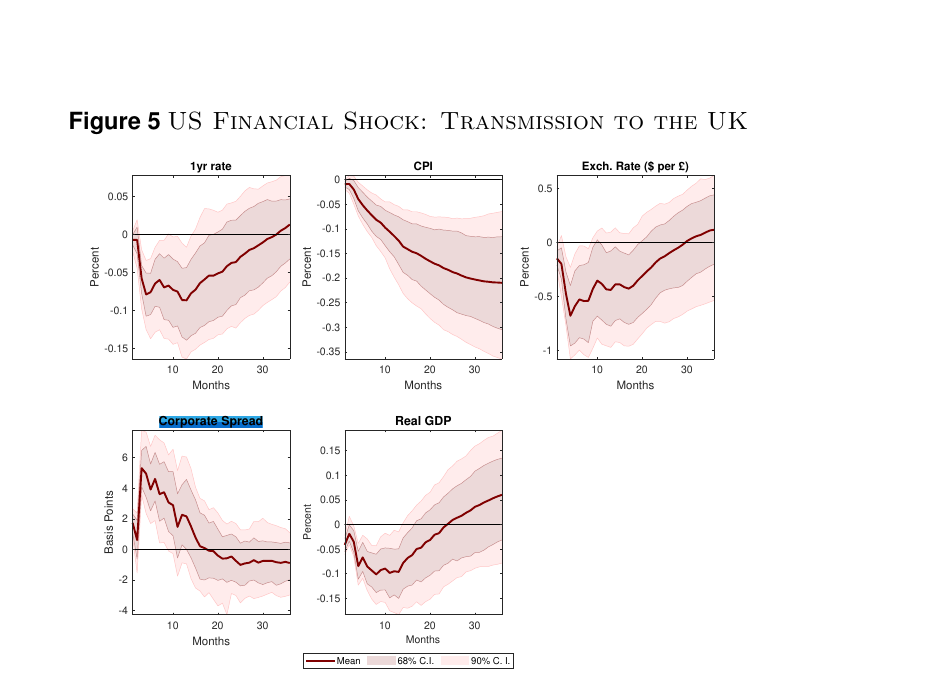
\includegraphics[width=0.85\linewidth]{images/fig5_usfin_uk.png}
\end{center}
\vspace{-0.4em}
\begin{itemize}\scriptsize
    \item U.K.\ corporate spreads rise to $\sim$5\,bp; real GDP and prices fall; sterling depreciates vs.\ the dollar.
    \item Happens \textbf{despite accommodating U.K.\ monetary policy} (1-yr gilt rate $\downarrow$ $\sim$10\,bp).
    \item \textcolor{blue}{$\boldsymbol{\Rightarrow}$} Evidence of an \textbf{international credit channel} of financial shocks.
\end{itemize}
\end{frame}


%-----------------------------------------------
% SLIDE 13 -- US MP shock to UK
%-----------------------------------------------
\begin{frame}{U.S.\ monetary-policy shock: transmission to the U.K.}
\begin{center}
    {\small \textbf{Figure 7} --- US Monetary Policy Shock: Transmission to the UK}\\[0.3em]
    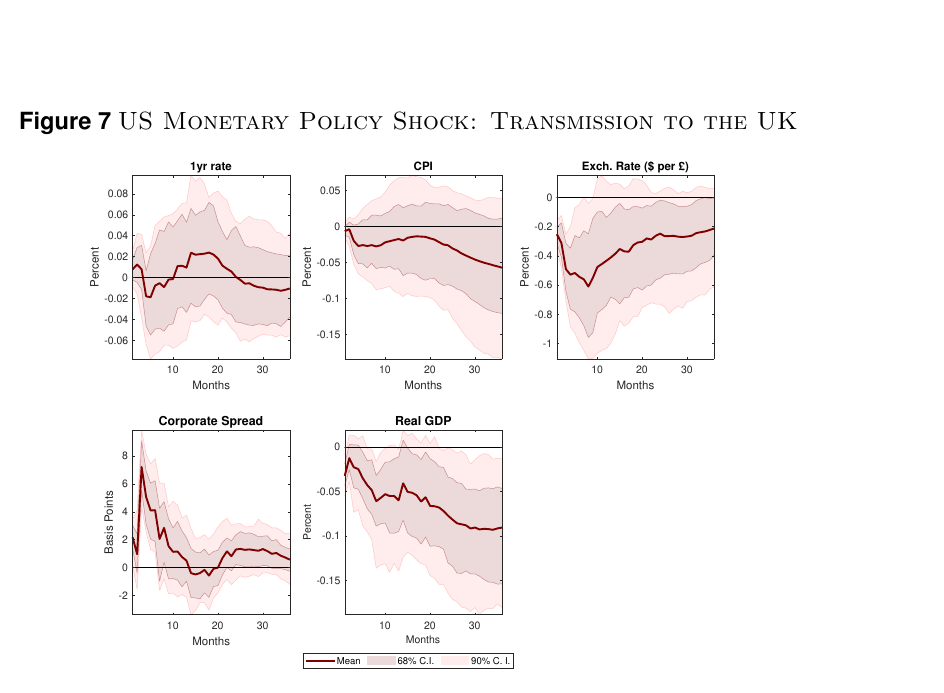
\includegraphics[width=0.85\linewidth]{images/fig7_usmp_uk.png}
\end{center}
\vspace{-0.4em}
\begin{itemize}\scriptsize
    \item U.S.\ MP tightening raises U.K.\ corporate spreads ($\sim$7\,bp); U.K.\ real GDP contracts; sterling depreciates.
    \item Consistent with the literature \textcolor{gray}{\scriptsize(Rey, 2016; Kalemli-\"Ozcan, 2019)}, with an improved identification that \textbf{explicitly controls for CBI effects}.
\end{itemize}
\end{frame}


%-----------------------------------------------
% SLIDE 14 -- CBI info shock to UK
%-----------------------------------------------
\begin{frame}{Central-bank information shock: transmission to the U.K.}
\begin{center}
    {\small \textbf{Figure 9} --- Fed Information Shock: Transmission to the UK}\\[0.3em]
    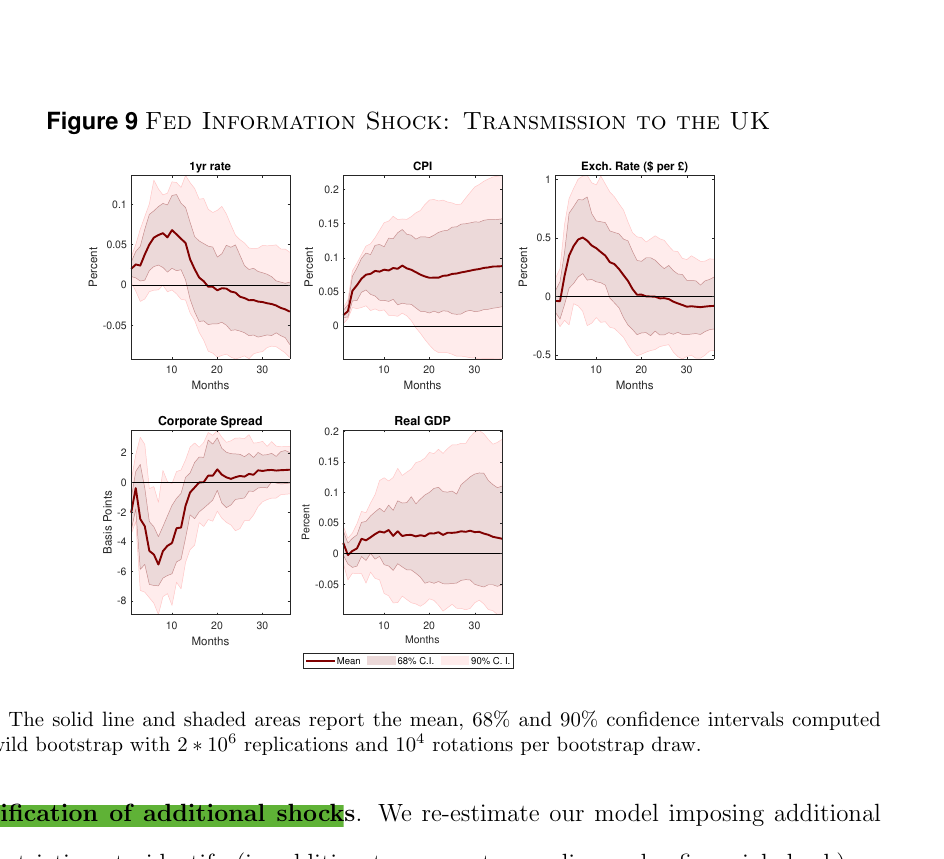
\includegraphics[width=0.8\linewidth]{images/fig9_cbi_uk.png}
\end{center}
\vspace{-0.4em}
\begin{itemize}\scriptsize
    \item A positive CBI shock (better-than-expected U.S.\ outlook) \textbf{compresses} U.S.\ credit spreads $\Rightarrow$ U.K.\ spreads fall, real GDP and prices rise.
    \item \textbf{Symmetry} of the ICC: the same mechanism that amplifies a bad shock also amplifies a good shock.
\end{itemize}
\scriptsize \textcolor{gray}{(Results hold when identifying an additional supply shock, using the inflation-targeting subsample from 1993:M1, excluding the Global Financial Crisis, and replacing GDP with unemployment.)}
\end{frame}


%===============================================
\section{Mechanism}
%===============================================

%-----------------------------------------------
% SLIDE 15 -- How credit spreads amplify international transmission
%-----------------------------------------------
\begin{frame}{How do credit spreads amplify international transmission?}
\begin{itemize}
    \item When an international credit channel is at work, domestic and foreign credit spreads not only \textbf{co-move} but also \textbf{amplify the real effects} of foreign shocks.
    \vspace{0.4em}
    \item \textbf{The mechanism -- a feedback loop:}
    \begin{itemize}\small
        \item Adverse shock $\rightarrow$ credit spreads rise,
        \item higher borrowing costs depress demand,
        \item lower demand reduces net worth,
        \item lower net worth raises spreads further.
    \end{itemize}
    \vspace{0.4em}
    \item With \textbf{internationally integrated balance sheets}, this loop operates across borders -- no-arbitrage in integrated financial markets creates tight linkages in macro dynamics across countries.
\end{itemize}
\end{frame}


%-----------------------------------------------
% SLIDE 17 -- Inspecting the mechanism
%-----------------------------------------------
\begin{frame}{Inspecting the mechanism}
\begin{center}
    {\small \textbf{Figure 10} --- Closing the International Credit Channel: The Response of Real GDP}\\[0.3em]
    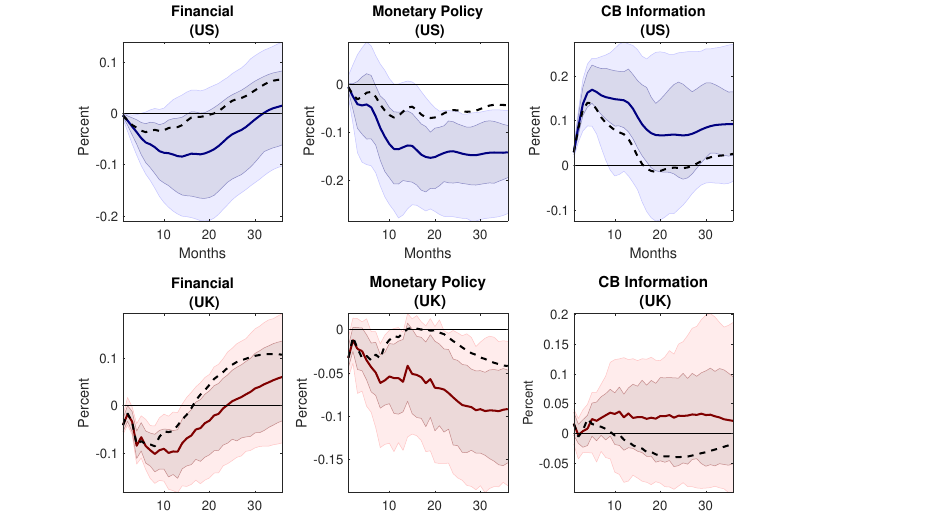
\includegraphics[width=0.82\linewidth]{images/fig10_closing_icc.png}
\end{center}
\vspace{-0.4em}
\begin{itemize}\scriptsize
    \item \textbf{Counterfactual holding credit spreads fixed:} GDP responses are \emph{smaller and less persistent} for all three shocks -- confirming the amplification role of credit spreads.
    \item \textbf{Alternative spread measures} (mortgage, Libor) respond counter-cyclically to all three shocks -- the ICC is not specific to corporate bond spreads.
\end{itemize}
\end{frame}


%-----------------------------------------------
% SLIDE 18 -- Discussion / role
%-----------------------------------------------
\begin{frame}{Discussion}
\begin{itemize}
    \item The \textbf{ICC is a general transmission channel}, operating through at least three distinct U.S.\ shocks:
    \begin{itemize}\small
        \item financial shocks, monetary-policy shocks, and central-bank information shocks.
    \end{itemize}
    \vspace{0.4em}
    \item The channel is \textbf{symmetric} -- same mechanism amplifies both contractionary and expansionary spillovers.
    \vspace{0.4em}
    \item \textbf{Implications:}
    \begin{itemize}\small
        \item Domestic monetary policy alone cannot insulate open economies from foreign financial conditions \textcolor{gray}{\scriptsize(cf.\ Rey's trilemma $\to$ dilemma)}.
        \item Credit-market stabilisation is first-order for open-economy macro policy.
    \end{itemize}
\end{itemize}
\end{frame}


%===============================================
\section{Conclusion}
%===============================================

%-----------------------------------------------
% SLIDE 19 -- Conclusion
%-----------------------------------------------
\begin{frame}{Conclusion}
\begin{itemize}
    \item \textbf{New identification} combining high-frequency IVs with a minimal sign restriction on the \emph{borrowing rate} -- cleanly separates financial shocks from aggregate-demand shocks.
    \vspace{0.4em}
    \item \textbf{International Credit Channel is pervasive:} U.S.\ financial, monetary-policy, and CBI shocks all transmit to the U.K.\ via credit spreads.
    \vspace{0.4em}
    \item \textbf{Credit spreads amplify} the international transmission of U.S.\ shocks -- closing them in a counterfactual materially dampens U.K.\ responses.
    \vspace{0.4em}
    \item \textbf{Policy takeaway:} in financially integrated economies, foreign credit conditions are a first-order driver of domestic macro dynamics.
\end{itemize}
\end{frame}


\begin{frame}
\centering
\Huge Thank you!
\vspace{1em}

\normalsize \textit{Comments and feedback welcome.}
\end{frame}


%------------------------------------------------
% APPENDIX / EXTRAS
%-----------------------------------------------
\appendix

\begin{frame}{Appendix: robustness}
\begin{itemize}\small
    \item Identify an additional supply shock.
    \item Restrict to the inflation-targeting subsample (from 1993:M1).
    \item Exclude the Global Financial Crisis window.
    \item Replace real GDP with unemployment.
\end{itemize}
\vspace{0.3em}
Main results unchanged across all alternatives.
\end{frame}

\begin{frame}{Appendix: alternative credit-spread measures}
\begin{center}
    {\small \textbf{Figure 11} --- UK's Response to US Financial Shock: Alternative Credit Spread Measures}\\[0.3em]
    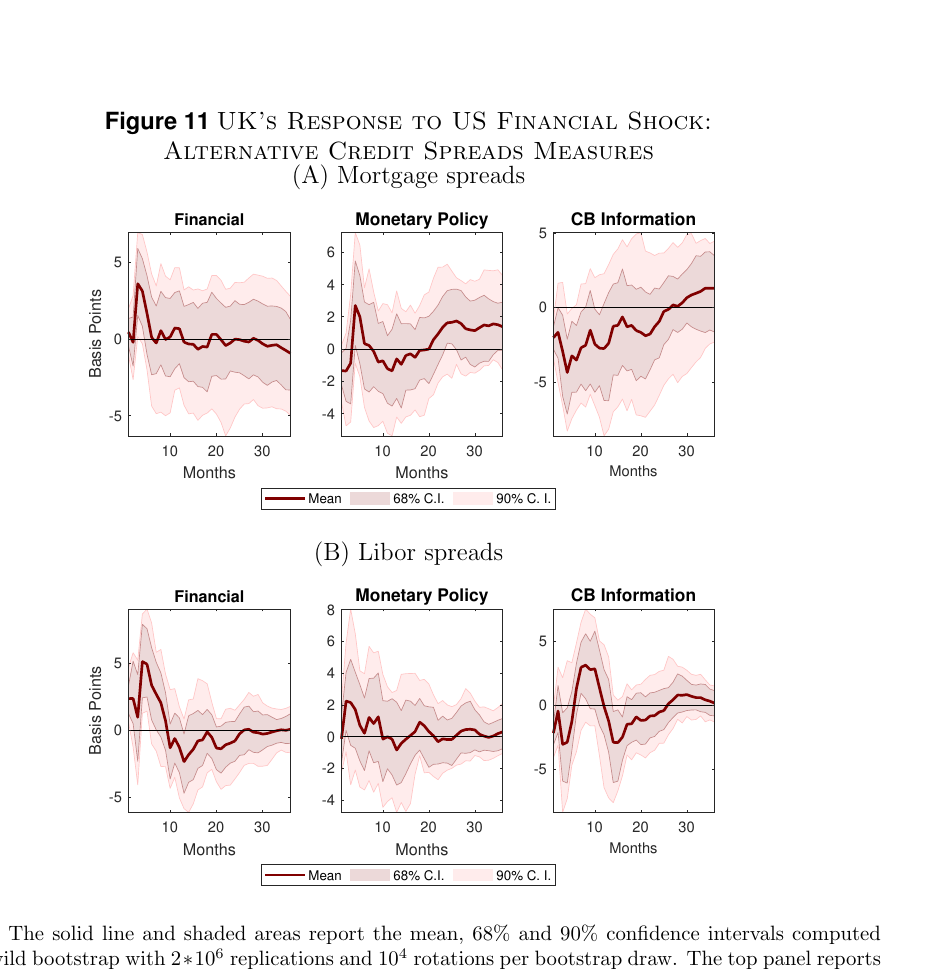
\includegraphics[width=0.78\linewidth]{images/fig11_alt_spreads.png}
\end{center}
\vspace{-0.3em}
{\scriptsize Top panel: mortgage spreads. Bottom panel: Libor spreads. Both respond counter-cyclically across the three shocks.}
\end{frame}

\end{document}
